\chapter{Implementation, integration and test plan}


\section{Development Process and Approach}

The system will be implemented, integrated, and tested following a bottom-up approach, 
starting from the model layer and progressively adding and testing the other components of the server architecture. 
This approach allows for the early validation of low-level functionalities, ensuring a solid foundation 
for higher-level components.

Both server-side and client-side components will be developed and tested simultaneously, 
but the focus will be on server-side components initially, due to their role as the backbone of the system. 
Incremental integration testing will be applied, aiming to identify and resolve bugs as soon as they emerge during 
the development process, minimizing the impact on subsequent stages.

To facilitate testing at different levels of the architecture, drivers will be employed to simulate higher-level 
components that are not yet implemented, while stubs will be used to mock the behavior of lower-level dependencies, 
such as external services or the database. This strategy ensures that individual components can be tested in isolation, 
while also validating their integration as part of the broader system.

This testing approach ensures that dependencies between components are carefully managed, 
leading to a robust and well-tested system at every level.


\section{Implementation and Integeration Plan}
This section will describe the implementation and integration plan of both sides of our system.



\subsection{Server Side}

In the first step, the Model (under the specified assumption of MVC pattern) and the
Query Service, will be implemented and unit tested with a Driver which will substitute
components which are not already implemented.

\begin{figure}[H]
    \centering
    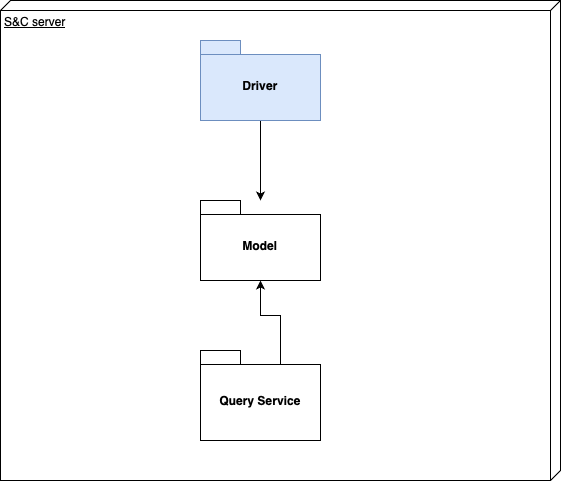
\includegraphics[width=300px]{../../assets/pakege-diagram/implementation_plan_1.png}
    \caption{I - Step}
\end{figure}


\newpage

In the second step, Authentication Service, Profile Manager, Recommendation Service, Enrolment Manager and
Internship Manager will be implemented and tested with a Driver which will substitute Request Dispatcher.

We will also use 3 Stub, which will substitute respectively: E-mail Service for Authentication Service, 
Suggestion Service for Profile Manager, Complaint Manager and Feedback Manager for Internship Manager.

\begin{figure}[H]
    \centering
    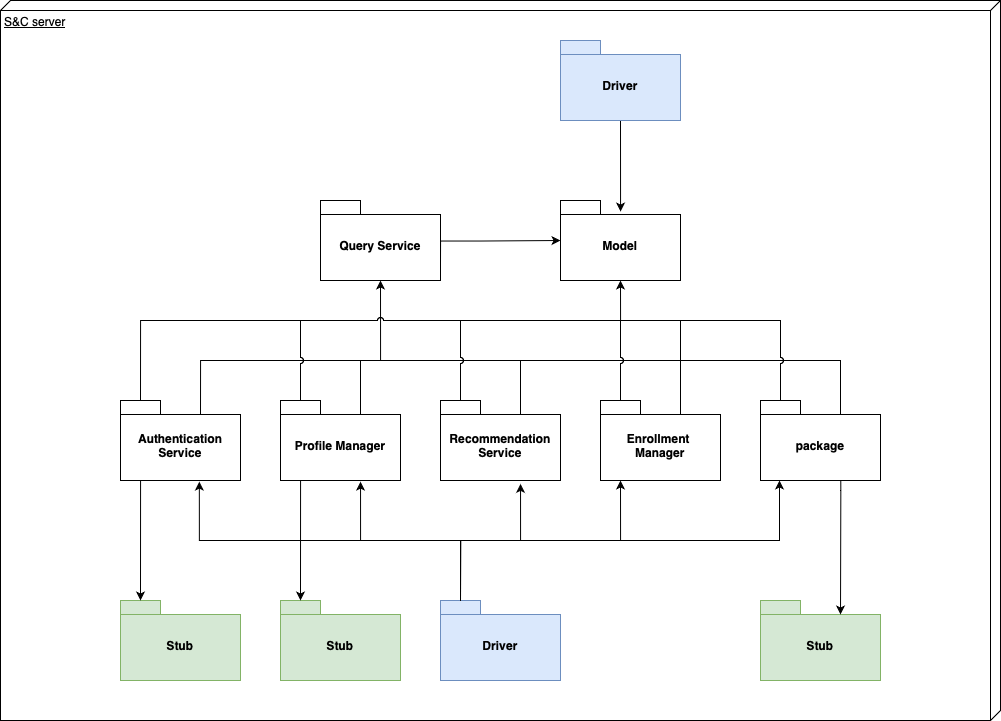
\includegraphics[width=450px]{../../assets/pakege-diagram/implementation_plan_2.png}
    \caption{II - Step}
\end{figure}


\newpage

In the third step, the Request Dispatcher will be implemented and tested, a Driver
will substitute the Web Server.

\begin{figure}[H]
    \centering
    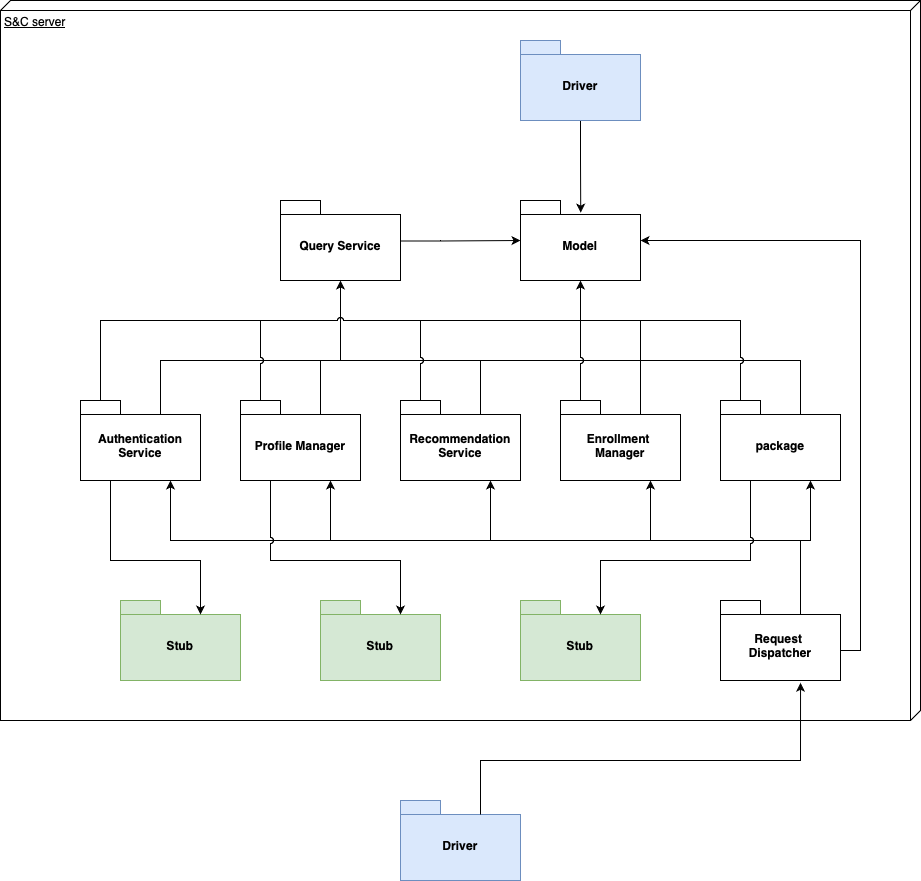
\includegraphics[width=450px]{../../assets/pakege-diagram/implementation_plan_3.png}
    \caption{III - Step}
\end{figure}


\newpage

In the fourth step, the last components of the server will be implemented, including Email Service, Suggestion Service,
Complaint Manager and Feedback Manager. 
A Stub will be used to simulate the behavior of the Email Server.

\begin{figure}[H]
    \centering
    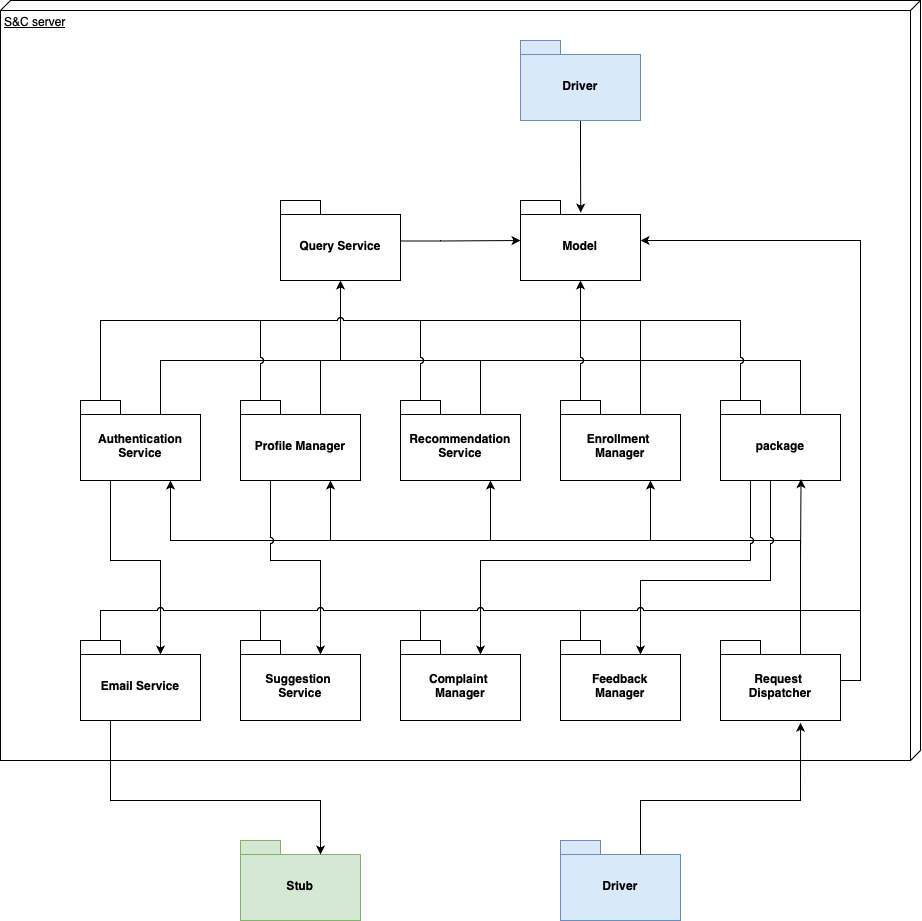
\includegraphics[width=450px]{../../assets/pakege-diagram/implementation_plan_4.png}
    \caption{IV - Step}
\end{figure}


\newpage

\subsection{Client Side}

Each component of the View is rigorously unit tested using a stub of the REST API, enabling
parallel development of the frontend and backend.

\begin{figure}[H]
    \centering
    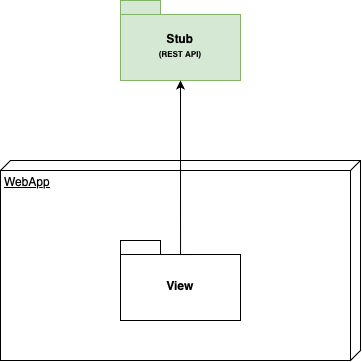
\includegraphics[width=180px]{../../assets/pakege-diagram/implementation_plan_5.png}
    \caption{View testing}
\end{figure}


\subsection{Final Test}

Once the implementations of the backend and of the frontend are finished, final tests can take place.

\begin{figure}[H]
    \centering
    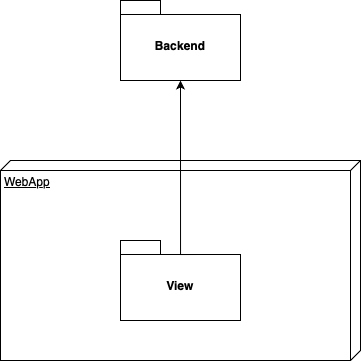
\includegraphics[width=180px]{../../assets/pakege-diagram/implementation_plan_6.png}
    \caption{View testing}
\end{figure}




